\section{Sensing the crest}
\label{sec:sensing}

\subsection{Why an accelerometer alone is not enough}
\label{sec:accel-only}

% add vector angle equation and use z hat notation for z vector
The robot has to know when it has crossed from the \ang{33.4} ramp onto the flat mesa, and it has to know this while speeding up and slowing down. An accelerometer reads acceleration along three basis vectors. At standstill, resultant acceleration vector retrieved is the gravity vector, from which it's trivial to calculate the robot's tilt: simply take the angle between the z vector and gravity vector.
However, when the robot accelerates along the ramp, the resultant vector ceases to be the gravity vector.

Along the ramp it reads $g \sin\ang{33.4} + a$ and across it $g \cos\ang{33.4}$, so the pitch it implies is
\begin{equation}
  \theta_\mathrm{apparent} = \arctan\!\left(\frac{g \sin\ang{33.4} + a}{g \cos\ang{33.4}}\right)
  \label{eq:apparent}
\end{equation}
Table~\ref{tab:apparent} shows the size of the error. Decelerating at \qty{3}{m/s^2} makes the ramp look like \ang{16}, below the \ang{18} threshold at which our robot decides it has crested.

\begin{table}[htbp]
  \centering
  \caption{Pitch an accelerometer alone reports on the \ang{33.4} ramp.}
  \label{tab:apparent}
  \begin{tabular}{@{}l cccccc@{}}
    \toprule
    $a$ along the ramp (\unit{m/s^2}) & $-3$ & $-2$ & $-1$ & 0 & $+1$ & $+2$ \\
    \midrule
    Apparent pitch (\unit{\degree}) & 16.3 & 22.5 & 28.2 & 33.4 & 38.0 & 42.1 \\
    \bottomrule
  \end{tabular}
\end{table}

% hold on wait a minute
% lowk why didn't we just solve this numerically for theta given that the acceleration in the x direction is known to be always 33deg up
% uhhhhhhhhh
A gyroscope measures rotation rate directly and is not fooled by linear acceleration, but turning its rate into an angle means integrating, and integration accumulates error. Ours read up to \qty{4.7}{\degree/s} with the robot at rest; over a \qty{5}{s} climb that offset alone would add \ang{23} of error.

\subsection{Complementary filter}
\label{sec:filter}

We combine the two sensors with a complementary filter that tracks the direction of gravity as a unit vector $\bm{u}$ in the sensor's frame, in the form of Mahony's explicit complementary filter~\cite{mahony}. Every \qty{20}{ms} the gyro rate $\bm{\omega}$ rotates the estimate, and the result is renormalized:
\begin{equation}
  \bm{u} \leftarrow \operatorname{normalize}\!\big(\bm{u} - (\bm{\omega} \times \bm{u})\,\Delta t\big)
  \label{eq:gyro-step}
\end{equation}
When the accelerometer reading $\hat{\bm{a}}$ can be trusted, the estimate is then pulled toward it with a time constant $T_c = \qty{1.5}{s}$:
\begin{equation}
  \bm{u} \leftarrow \operatorname{normalize}\!\left(\bm{u} + \frac{\Delta t}{T_c}\left(\frac{\hat{\bm{a}}}{|\hat{\bm{a}}|} - \bm{u}\right)\right)
  \label{eq:accel-step}
\end{equation}
The accelerometer is trusted only while its reading is within \qty{8}{\percent} of \qty{1}{g}, the rotation rate is below \qty{30}{\degree/s}, and the motor commands have been steady for \qty{0.6}{s}. In every other moment the estimate follows the gyro alone. The gyro offset is averaged over 50 readings with the robot at rest and subtracted from every reading after that. A two-step calibration (robot level, then nose up) gives the robot its own up and forward directions, from which it computes pitch.

\subsection{Requirement and test}
\label{sec:pitch-test}

The autopilot decides it has crested when the pitch stays below \ang{18} for \qty{40}{ms}, and on the mesa it counts anything within \ang{\pm 6} as level. The estimate therefore must not read more than \ang{15} low while climbing the \ang{33.4} ramp, and must be within \ang{\pm 6} at rest. \tbd{Confirm these were the thresholds used in the contest.}

To test this we used the hill itself as ground truth: anywhere on the ramp the true pitch is \ang{33.4}, and on the mesa it is \ang{0}. We logged both the accelerometer-only and the fused pitch through three full autonomous runs (Fig.~\ref{fig:pitch}, Table~\ref{tab:pitch}). Climbing, the accelerometer alone was off by up to \ang{122}, while the fused estimate never read more than \ang{4.5} from the true angle, well inside the \ang{15} the crest test allows. At rest, both were within \ang{4} on the mesa, inside the \ang{\pm 6} level band.

\begin{figure}[htbp]
  \centering
  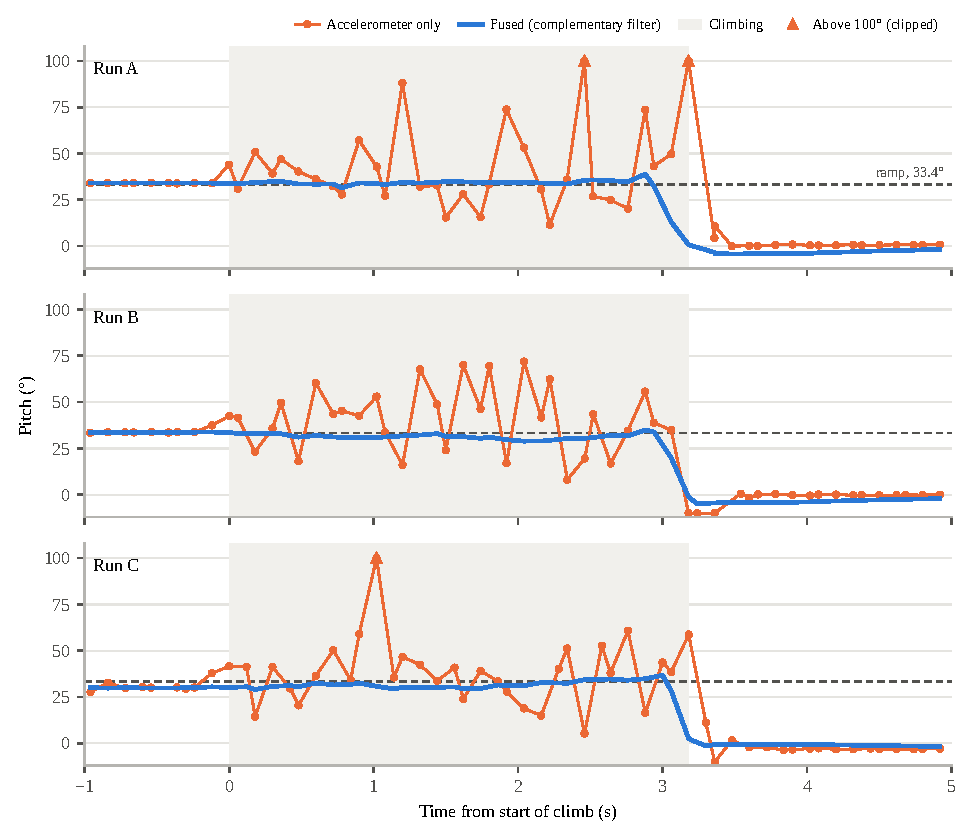
\includegraphics[width=0.92\textwidth]{fig11_pitch.pdf}
  \caption{Pitch during three autonomous climbs. Under full power the accelerometer alone reads anywhere from \ang{5} to over \ang{150}, while the fused estimate stays within \ang{4.5} of the true \ang{33.4} until the crest.}
  \label{fig:pitch}
\end{figure}

\begin{table}[htbp]
  \centering
  \caption{Pitch error against the known hill angle (\ang{33.4} on the ramp, \ang{0} on the mesa). Climbing uses all three runs; the rest rows use Runs A and B, since Run C started off the ramp face.}
  \label{tab:pitch}
  \begin{tabular}{@{}l cc cc@{}}
    \toprule
    & \multicolumn{2}{c}{Accelerometer only} & \multicolumn{2}{c}{Fused} \\
    \cmidrule(lr){2-3}\cmidrule(l){4-5}
    Condition & Max.\ error & RMS & Max.\ error & RMS \\
    \midrule
    At rest on the ramp       & \ang{0.8}   & \ang{0.5}  & \ang{0.6} & \ang{0.5} \\
    Climbing under full power & \ang{121.7} & \ang{24.0} & \ang{4.5} & \ang{2.1} \\
    At rest on the mesa       & \ang{0.8}   & \ang{0.5}  & \ang{3.9} & \ang{1.6} \\
    \bottomrule
  \end{tabular}
\end{table}
